% Slides for 2024-08-20
% To create a slide, use the following:
% \begin{frame}{TITLE}
%     BODY
% \end{frame}

\begin{frame}{Loss with different noises}
    \centering
    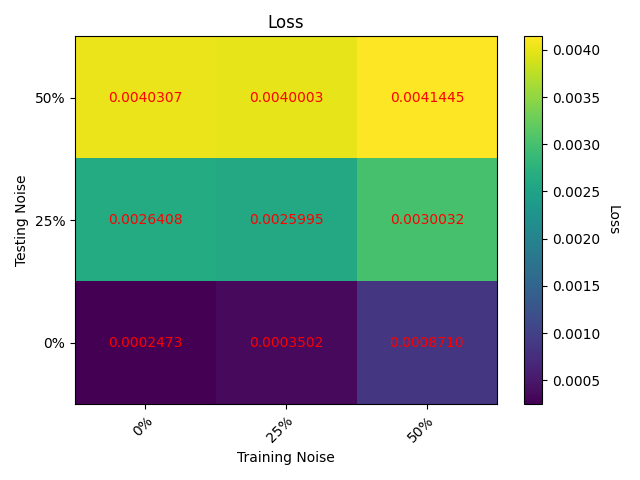
\includegraphics[width = 0.6\linewidth]{images/Loss.png}
\end{frame}

\begin{frame}{Loss with different noises}
    \centering
    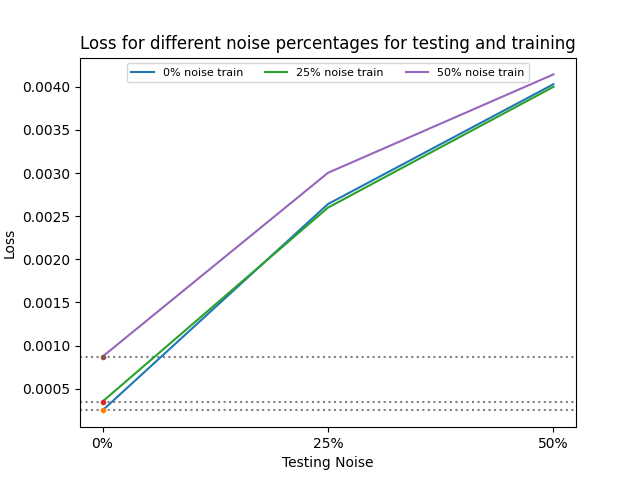
\includegraphics[scale = 0.5]{images/Loss for different noise percentages for testing and training.png}
\end{frame}


\begin{frame}{To-do}
    \begin{itemize}
        \item try different noises with a smaller model
    \end{itemize}
\end{frame}

% To create a slide with a graphic:
% 1. Add the graphic to this folder (named picture.png)
% 2. Use the following:
% \begin{frame}{TITLE}
%     \centering
%     \includegraphics[height=0.7\textheight,width=0.7\textwidth,keepaspectratio]{picture.png}
% \end{frame}

% To create a slide with two columns, use the following:
% \begin{frame}{TITLE}
%     \begin{columns}
%         \begin{column}{0.5\textwidth}
%             COLUMN 1 BODY
%         \end{column}
%         \begin{column}{0.5\textwidth}
%             COLUMN 2 BODY
%         \end{column}
%     \end{columns}
% \end{frame}
